\documentclass{article}

\usepackage[english]{babel}

% Set page size and margins
\usepackage[a4paper,top=2cm,bottom=2cm,left=3cm,right=3cm,marginparwidth=1.75cm]{geometry}

% Useful packages
\usepackage{amsmath}
\usepackage{graphicx}
\graphicspath{{./images/}}
\usepackage[colorlinks=true, allcolors=blue]{hyperref}


\title{Weather and Crops: An Exploration of Agrotech}


\begin{document}
\maketitle

\begin{table}[h]
    \centering
    \begin{tabular}{ll}
        Registration number: & \textcolor{red}{2100374}\\
        Project: & \textcolor{red}{Agrotech}\\
        Link to GitHub: & \url{https://github.com/rigovm101/CE888_DataScience/tree/main/Project}\\
    \end{tabular}
\end{table}

\begin{table}[h]
    \centering
    \begin{tabular}{lc}
        Executive summary (max.\ 250 words) & \textcolor{red}{73}\\
        Introduction (max.\ 600 words) & \textcolor{red}{273}\\
        Data (max.\ 300 words/dataset) & \textcolor{red}{249}\\
        Methodology (max.\ 600 words) & \textcolor{red}{113}\\
        Results and Discussion (max.\ 1000 words combined) & \textcolor{red}{200}\\
        Conclusions (max.\ 500 words) & \textcolor{red}{101}\\
        \hline
        Total word count & \textcolor{red}{1,009}\\
    \end{tabular}
\end{table}

\tableofcontents

\clearpage

\begin{abstract}
This project aims to build a Machine Learning model capable of using
the Agrotech dataset to predict the growth of crops using historic
weather information, as well as information about the planting process
and the crops themselves. The \emph{ScikitLearn} Python Library
was used to develop and test four Machine Learning models, with the
best model achieving a \(R^2\) score of 0.82, with a RMSE score
of 30.73 on the prediction of its three labels.
\end{abstract}


\section{Introduction}
Waste exists in a lot industries. With the increase on population and changes in consumption
habits, companies have had to adapt to these changes and cut down on waste. Another rapidly
changing factor in todays world is weather. Climate change has brought a lot of uncertainty
to our daily activities. An industry which is at the intersection of these two topics is
the food industry, specifically the farming industry.

Machine Learning is a somewhat recent, it's been around the 1980s \cite{mlBook}. It has
provided many tools and models to identify patterns and solve problems \cite{mlBookTwo}.
Relying primarily on data, Machine Learning is a strong candidate to fight this problem of
food waste.

There are many drivers which cause food waste along the supply chain, with many of these
being partially responsible for food waste. Bad practices come from innapropiate choice of
crop varieties, all the way to poor water and nutrient management \cite{foodLoss}.
Not only farms are responsible, but also supermarkets. As noted by a study done in Brazil,
one of the main causes for food waste is ”inneffective stock control management” \cite{brazfood}.
A report here in the UK also estimates that around 40.7\% of the fresh products gets wasted or not
completely used \cite{ukarticle}. Many scientist belive that effective planning and control
over the production can help reduce drastically the amount of wasted food \cite{savingFood}.

While it's impossible (or at least very unlikely) to predict weather data to better plan
the production of crops, Machine Learning model can provide with an estimate of weather
conditions, using data available online. The team is optimistic to building a useful model
capable in assisting in the planing phases of crop production.

\section{Data}

The project supervisor was the person responsible for providing the team with the dataset.
Given it's sensitivity and confidentiality, this dataset is not publicly. As the main
repository is kept public for research purpuses, the dataset will be kept locally. This
dataset contains information about crops and weather. Table \ref{table:1} contains
information about each individual sheet on the \emph{.csv} file.

\begin{table}[h]
    \centering
    \begin{tabular}{ | c | c |}
        \hline
        Plants & Information about the plants \\
        \hline
        Flight Dates & Information about the flights \\
        \hline
        Planting & Additional information about the plants \\
        \hline
        Weather & Historical weather information \\
        \hline
    \end{tabular}
    \caption{Table with the information per sheet Agrotech}
    \label{table:1}
\end{table}

The sheet \emph{Plants} contains our labels to predict, under the column names
\emph{Head Weight, Polar Diamter and Radial Diameter}. The type of data in these
columns is Float and contain some NULL values. The data consists of 4859 rows. Rows with
missing values on the label columns were dropped, as well as rows marked by the \emph{Remove}
column (which was also removed).

The \emph{Flight Dates} sheet only contained the Flight Dates for specific Batch Numbers.
This sheet was merged with the \emph{Plants} sheet to fill in missing dates. The \emph{Planting}
sheet contained additional information about each Batch. It was also merged with the previous
sheets. Lastly the \emph{Weather} sheet contains historic weather data.

Features were created from the \emph{Weather} sheet. We used the Plant Date and Flight
Date to extract the weather conditions a certain batch was subject to. Some of the features
extracted were \emph{Mean Solar Radiation, Total Precipitation, Mean Air Temperature and
Humidity}.

The resulting dataset consists of 18 features and 3 labels, with 3236 rows. Most of the features
are numerical values, with only one categorical feature. The data was standarised to reduce
size difference in dimensions.

\section{Methodology}

With the pre-processing part of the project finished, we now turn towards the actual
training of the model. The team used the \emph{ScikitLearn} library in Python to implement
the Machine Learning models. The selected models are:

\begin{itemize}
    \item Linear Regression
    \item Decision Tree
    \item Random Forest Regressor
    \item Gradient Booster Regression
\end{itemize}

Since this is a Multi-Output Regression problem, these models will be wrapped in a
\emph{MultiOutputRegressor} class. This will allow us to build and test the model to
predict more than one label at a time. Figure \ref{figure:1} shows the system architecture
of the project.

\begin{figure}[h]
    \centering
    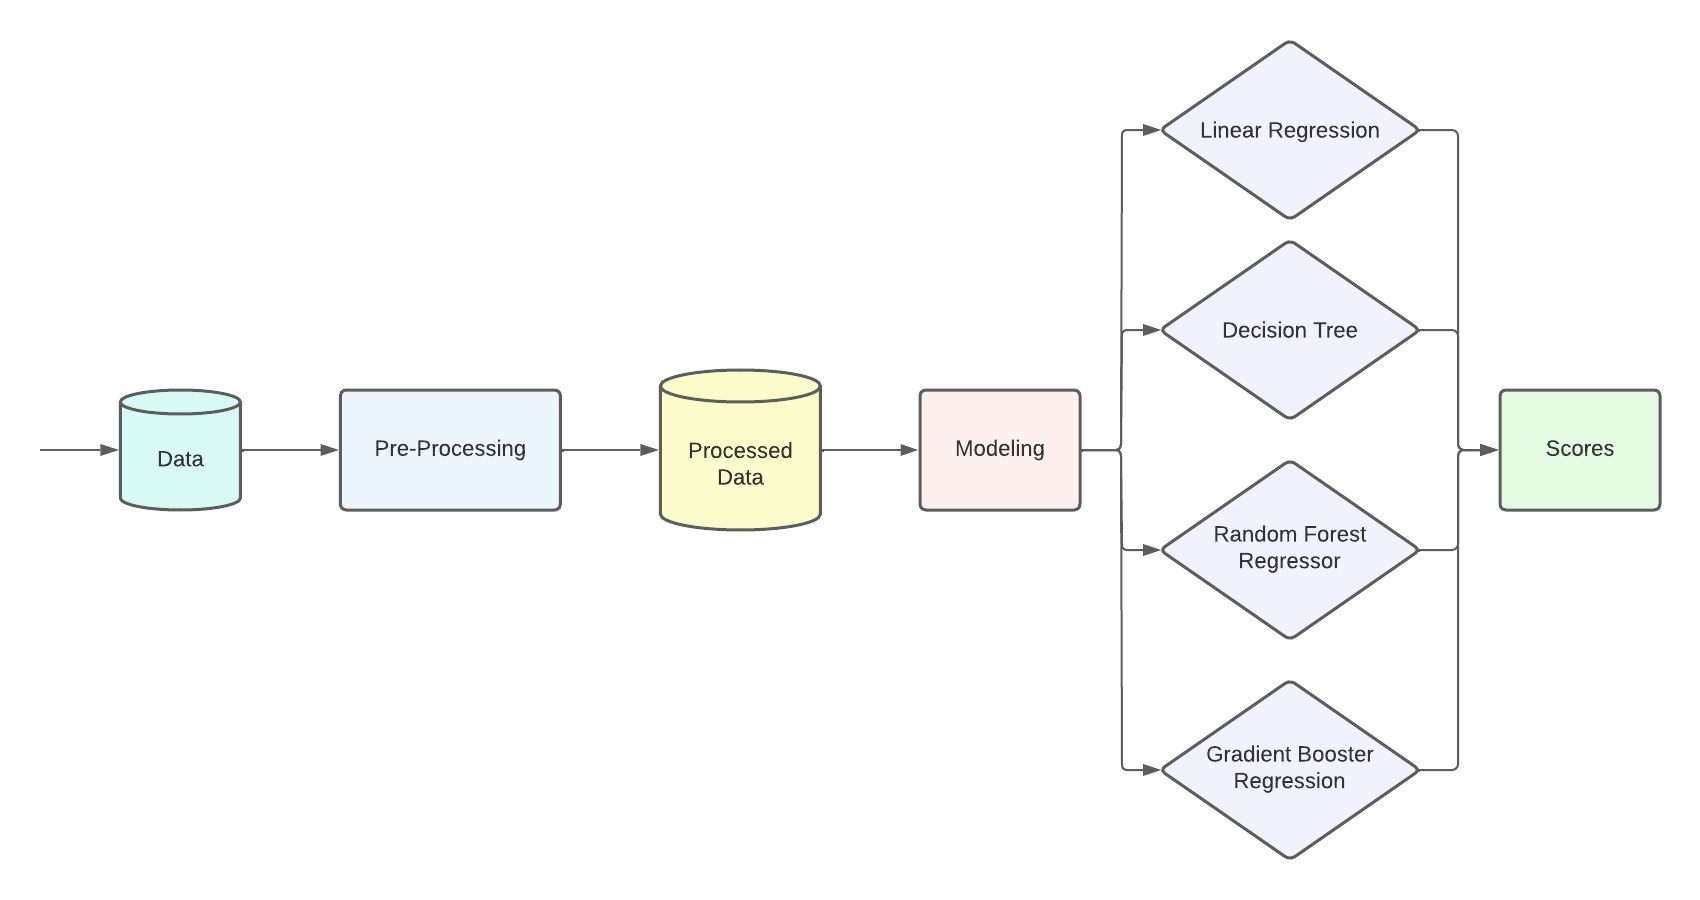
\includegraphics[width=\textwidth]{ProjectDiagram.png}
    \caption{Project Diagram}
    \label{figure:1}
\end{figure}

All the models will be evaluated using 10-fold cross-validation. The metrics to be used
for evaluation will be Root Mean Squared Error (RMSE) and \(R^2\).

\section{Results}

The results of the training can be seen in Table \ref{table:2}. Figures
\ref{figure:2} and \ref{figure:3} also provides comparison between the models developed.

\begin{table}[h]
    \centering
    \begin{tabular}{ | c | c | c |}
        \hline
        ML Model & \(R^2\) & RMSE \\
        \hline
        \hline
        Linear Regression & 0.68 & 38.03 \\
        \hline
        Decision Tree & 0.64 & 44.36 \\
        \hline
        Random Forest Regression & 0.82 & 32.34 \\
        \hline
        Gradient Booster Regression & 0.82 & 30.73 \\
        \hline
    \end{tabular}
    \caption{Performance per Model}
    \label{table:2}
\end{table}

\begin{figure}[h]
    \centering
    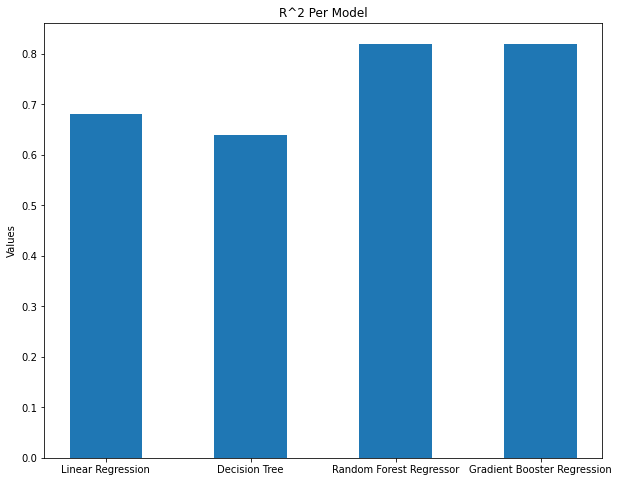
\includegraphics[width=\textwidth]{R2Values.png}
    \caption{\(R^2\) Values per Model}
    \label{figure:2}
\end{figure}

\begin{figure}[h]
    \centering
    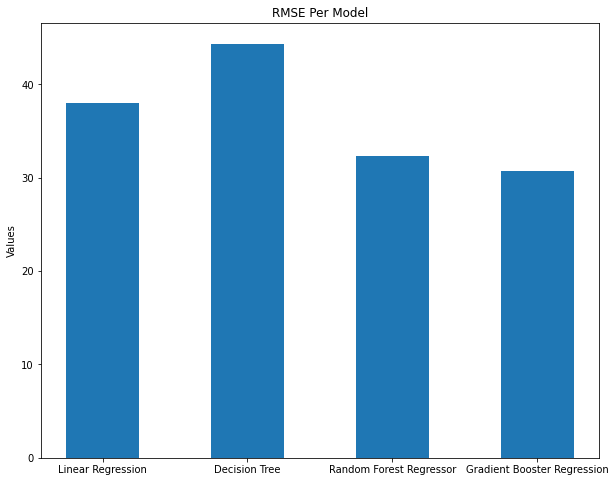
\includegraphics[width=\textwidth]{RMSEValues.png}
    \caption{RMSE Values per Model}
    \label{figure:3}
\end{figure}

\section{Discussion}

The Linear Regression model achieved an \(R^2\) score of 0.68 and an RMSE score of
38.03. Since there are no hyper-parameters in this model no tuning was made.

The Decision Tree model achieved an \(R^2\) score of 0.64 and an RMSE score of
44.36. The \emph{max\_depth} parameter was modified during the training of the model,
but no significant improvements came from this tuning.

The Random Forest Regression model achieved an \(R^2\) score of 0.82 and an RMSE score of
32.34. The The \emph{n\_estimators} parameter was modified in the ranges of (50, 100, 150, 200)
with no improvements in the scores but significant increase in the training time the higher
the number of estimators, therefore the default value of 100 was used.

The Gradient Booster Regression model achieved an \(R^2\) score of 0.82 and as RMSE score of
30.73. The \emph{learning\_rate} parameter was tuned but saw no significant
improvement on the scores. The \emph{nestimators} parameter was also tuned,
but saw no actual improvement on the scores.

Given the data we determied the best model is the Gradient Booster Regression.
Figure \ref{figure:2} provides a comparison between the \(R^2\) score
among the models, while Figure \ref{figure:3} provides a comparison between
the RMSE scores among the models.

\section{Conclusions}
The approach used by the team involved using cummulative information from the weather conditions
the crop had already been exposed to. This approach doesn't take into account possible
future conditions the crops has still yet to face before it's Check Date. While its
impossible to accurately predict the weather conditions, historic data from previous
years might be useful to improve the performance of the model. This is a potential avenue
for future research.

The model built for this project can be used for some rough estimates to help Agrotech
better plan the production of their crops and help reduce food waste.

\pagebreak

\bibliographystyle{abbrv}
\bibliography{sample}

\end{document}